% Options for packages loaded elsewhere
% Options for packages loaded elsewhere
\PassOptionsToPackage{unicode}{hyperref}
\PassOptionsToPackage{hyphens}{url}
\PassOptionsToPackage{dvipsnames,svgnames,x11names}{xcolor}
%
\documentclass[
]{article}
\usepackage{xcolor}
\usepackage[lmargin=1.2in,rmargin=1.5in,tmargin=1.5in,bmargin=1.2in]{geometry}
\usepackage{amsmath,amssymb}
\setcounter{secnumdepth}{-\maxdimen} % remove section numbering
\usepackage{iftex}
\ifPDFTeX
  \usepackage[T1]{fontenc}
  \usepackage[utf8]{inputenc}
  \usepackage{textcomp} % provide euro and other symbols
\else % if luatex or xetex
  \usepackage{unicode-math} % this also loads fontspec
  \defaultfontfeatures{Scale=MatchLowercase}
  \defaultfontfeatures[\rmfamily]{Ligatures=TeX,Scale=1}
\fi
\usepackage{lmodern}
\ifPDFTeX\else
  % xetex/luatex font selection
\fi
% Use upquote if available, for straight quotes in verbatim environments
\IfFileExists{upquote.sty}{\usepackage{upquote}}{}
\IfFileExists{microtype.sty}{% use microtype if available
  \usepackage[]{microtype}
  \UseMicrotypeSet[protrusion]{basicmath} % disable protrusion for tt fonts
}{}
\makeatletter
\@ifundefined{KOMAClassName}{% if non-KOMA class
  \IfFileExists{parskip.sty}{%
    \usepackage{parskip}
  }{% else
    \setlength{\parindent}{0pt}
    \setlength{\parskip}{6pt plus 2pt minus 1pt}}
}{% if KOMA class
  \KOMAoptions{parskip=half}}
\makeatother
% Make \paragraph and \subparagraph free-standing
\makeatletter
\ifx\paragraph\undefined\else
  \let\oldparagraph\paragraph
  \renewcommand{\paragraph}{
    \@ifstar
      \xxxParagraphStar
      \xxxParagraphNoStar
  }
  \newcommand{\xxxParagraphStar}[1]{\oldparagraph*{#1}\mbox{}}
  \newcommand{\xxxParagraphNoStar}[1]{\oldparagraph{#1}\mbox{}}
\fi
\ifx\subparagraph\undefined\else
  \let\oldsubparagraph\subparagraph
  \renewcommand{\subparagraph}{
    \@ifstar
      \xxxSubParagraphStar
      \xxxSubParagraphNoStar
  }
  \newcommand{\xxxSubParagraphStar}[1]{\oldsubparagraph*{#1}\mbox{}}
  \newcommand{\xxxSubParagraphNoStar}[1]{\oldsubparagraph{#1}\mbox{}}
\fi
\makeatother


\usepackage{longtable,booktabs,array}
\usepackage{calc} % for calculating minipage widths
% Correct order of tables after \paragraph or \subparagraph
\usepackage{etoolbox}
\makeatletter
\patchcmd\longtable{\par}{\if@noskipsec\mbox{}\fi\par}{}{}
\makeatother
% Allow footnotes in longtable head/foot
\IfFileExists{footnotehyper.sty}{\usepackage{footnotehyper}}{\usepackage{footnote}}
\makesavenoteenv{longtable}
\usepackage{graphicx}
\makeatletter
\newsavebox\pandoc@box
\newcommand*\pandocbounded[1]{% scales image to fit in text height/width
  \sbox\pandoc@box{#1}%
  \Gscale@div\@tempa{\textheight}{\dimexpr\ht\pandoc@box+\dp\pandoc@box\relax}%
  \Gscale@div\@tempb{\linewidth}{\wd\pandoc@box}%
  \ifdim\@tempb\p@<\@tempa\p@\let\@tempa\@tempb\fi% select the smaller of both
  \ifdim\@tempa\p@<\p@\scalebox{\@tempa}{\usebox\pandoc@box}%
  \else\usebox{\pandoc@box}%
  \fi%
}
% Set default figure placement to htbp
\def\fps@figure{htbp}
\makeatother





\setlength{\emergencystretch}{3em} % prevent overfull lines

\providecommand{\tightlist}{%
  \setlength{\itemsep}{0pt}\setlength{\parskip}{0pt}}



 


\makeatletter
\@ifpackageloaded{caption}{}{\usepackage{caption}}
\AtBeginDocument{%
\ifdefined\contentsname
  \renewcommand*\contentsname{Table of contents}
\else
  \newcommand\contentsname{Table of contents}
\fi
\ifdefined\listfigurename
  \renewcommand*\listfigurename{List of Figures}
\else
  \newcommand\listfigurename{List of Figures}
\fi
\ifdefined\listtablename
  \renewcommand*\listtablename{List of Tables}
\else
  \newcommand\listtablename{List of Tables}
\fi
\ifdefined\figurename
  \renewcommand*\figurename{Figure}
\else
  \newcommand\figurename{Figure}
\fi
\ifdefined\tablename
  \renewcommand*\tablename{Table}
\else
  \newcommand\tablename{Table}
\fi
}
\@ifpackageloaded{float}{}{\usepackage{float}}
\floatstyle{ruled}
\@ifundefined{c@chapter}{\newfloat{codelisting}{h}{lop}}{\newfloat{codelisting}{h}{lop}[chapter]}
\floatname{codelisting}{Listing}
\newcommand*\listoflistings{\listof{codelisting}{List of Listings}}
\makeatother
\makeatletter
\makeatother
\makeatletter
\@ifpackageloaded{caption}{}{\usepackage{caption}}
\@ifpackageloaded{subcaption}{}{\usepackage{subcaption}}
\makeatother
\usepackage{bookmark}
\IfFileExists{xurl.sty}{\usepackage{xurl}}{} % add URL line breaks if available
\urlstyle{same}
\hypersetup{
  colorlinks=true,
  linkcolor={blue},
  filecolor={Maroon},
  citecolor={Blue},
  urlcolor={Blue},
  pdfcreator={LaTeX via pandoc}}


\author{}
\date{}
\begin{document}


\begin{center}
{\Large \textbf{Deploying Real Time Object Detection Inference Systems}} \\
\vspace{1em}
Yves Kreimerman, 2025
\end{center}

\textbf{Abstract.} Computer vision is a field in machine learning that
aims to understand a give picture, identify what's going on and classify
those into classes(patterns) it understands. There are couple of main
fields in the computer vision world, those being:

\begin{enumerate}
\def\labelenumi{\arabic{enumi}.}
\tightlist
\item
  \textbf{Classification} - The model classifies a whole picture into
  classes. It is possible for the model to classify the picture as
  multiple classes(Multi-Label Classification), or one class, being the
  most dominant(Multi-Class Classification) \newline
\item
  \textbf{Object Detection} - The model omits a series of boxes around
  various object it identifies(based on the data it was trained),
  pointing to the coordinates where the object is found on the picture.
  \newline
\item
  \textbf{Semantic Segmentation} - The model identifies pixels as part
  of a class, but does not distinct between different objects sharing
  the same class \newline
\item
  \textbf{Instance Segmentation}- The model identifies pixels as part of
  a class, and has the distinction between objects. it is able to
  distinct two objects from the same class that are nearby.
\end{enumerate}

\section{1. Introduction}\label{introduction}

Live streaming video is a broad subject, of producing a live video feed
which is constantly broadcasted from various sources, with consumers
watching on the other end. Live streaming is usually split into couple
of main categories, the main ones being:

\begin{table}[h!]
\centering
\begin{tabular}{|l|c|l|}
\hline
\textbf{Type} & \textbf{Delay Range (Seconds)} & \textbf{Use} \\
\hline
WebRTC & 0.5 - 2 & Real Time (video calls, surveillance) \\
\hline
Broadcast Live & 2 - 5 & TV (News, Sports) \\
\hline
RTMP/HLS & 5 - 30+ & Live Media (Youtube, Twitch) \\
\hline
\end{tabular}
\caption{Main categories of live streaming}
\end{table}

Having Machine Learning fit model into the chain of live streaming can
be difficult, as it requires us to fit under very slim time constraints.
\newline With Real Time being our main subject, we will go over the
constraints we should take into count, and how they project on our
system design:

\begin{enumerate}
\def\labelenumi{\arabic{enumi}.}
\tightlist
\item
  \textbf{Source Capture \& Extraction of raw frame} - Getting raw
  frames from source, before any manipulations - \underline{30ms}
  \newline
\item
  \textbf{Machine Learning Inference} - Processing, model inference,
  postprocessing \newline
\item
  \textbf{Video encoding \& Processing} - Processing frames into actual
  video, encoding to various formats(e.g.~H264) - \underline{20ms}
  \newline
\item
  \textbf{Network Transport} - Transporting the processed video to
  consumer(Over LAN/WAN) - \underline{100ms-150ms} \newline
\item
  \textbf{Consumer Decoding \& Display} - Displaying the video to the
  end consumer via streaming platform - \underline{100ms-130ms}
\end{enumerate}

The numbers shown are for an ideal scenario, and in reality numbers are
much higher. That requires us to fit under very low constraints, ideally
around \textbf{15ms-75ms}, depending on video frame rate and network
throughput. \newpage{}

\section{3. Methodology}\label{methodology}

Having tight time constraints to take into consideration, we would have
to design a low-latency, high throughput system, that can serve as many
video sources as possible, while utilizing the most from the given
resources.

\subsection{3.1 Model Precision}\label{model-precision}

With the goal of minimizing latency of inferance, and maximizing
processing throughput, we need a way to optimize the given ML models and
squeeze the best preformance out of those. \newline By default, machine
learning models use FP32(Floating point 32) datatypes for weights and
inputs/outputs by default, allowing higher precision for training,
therefore maximizing accuracy. When running inference on the same
models, we don't necessarily need all that precision and can
``compromise'' on lower floating points, i.e.~FP16. FP16 should give us
much better preformance, while almost not compromising on accuracy.
\newline We first want to test all model versions for accuracy,
determine how lossy is the conversion of floating points and is
compromising on floating points even worth it. \newline We will do so
with a pre-made evaluation script, while models are evaluated on MS-COCO
Val 2017 dataset, for consistency purposes(all models are trained on the
same data too). \newline The goal is to demonstrate how one model
compares to another, so the actual performance of the model(how well it
performs on the data) is trivial.

\begin{figure}[H]

{\centering 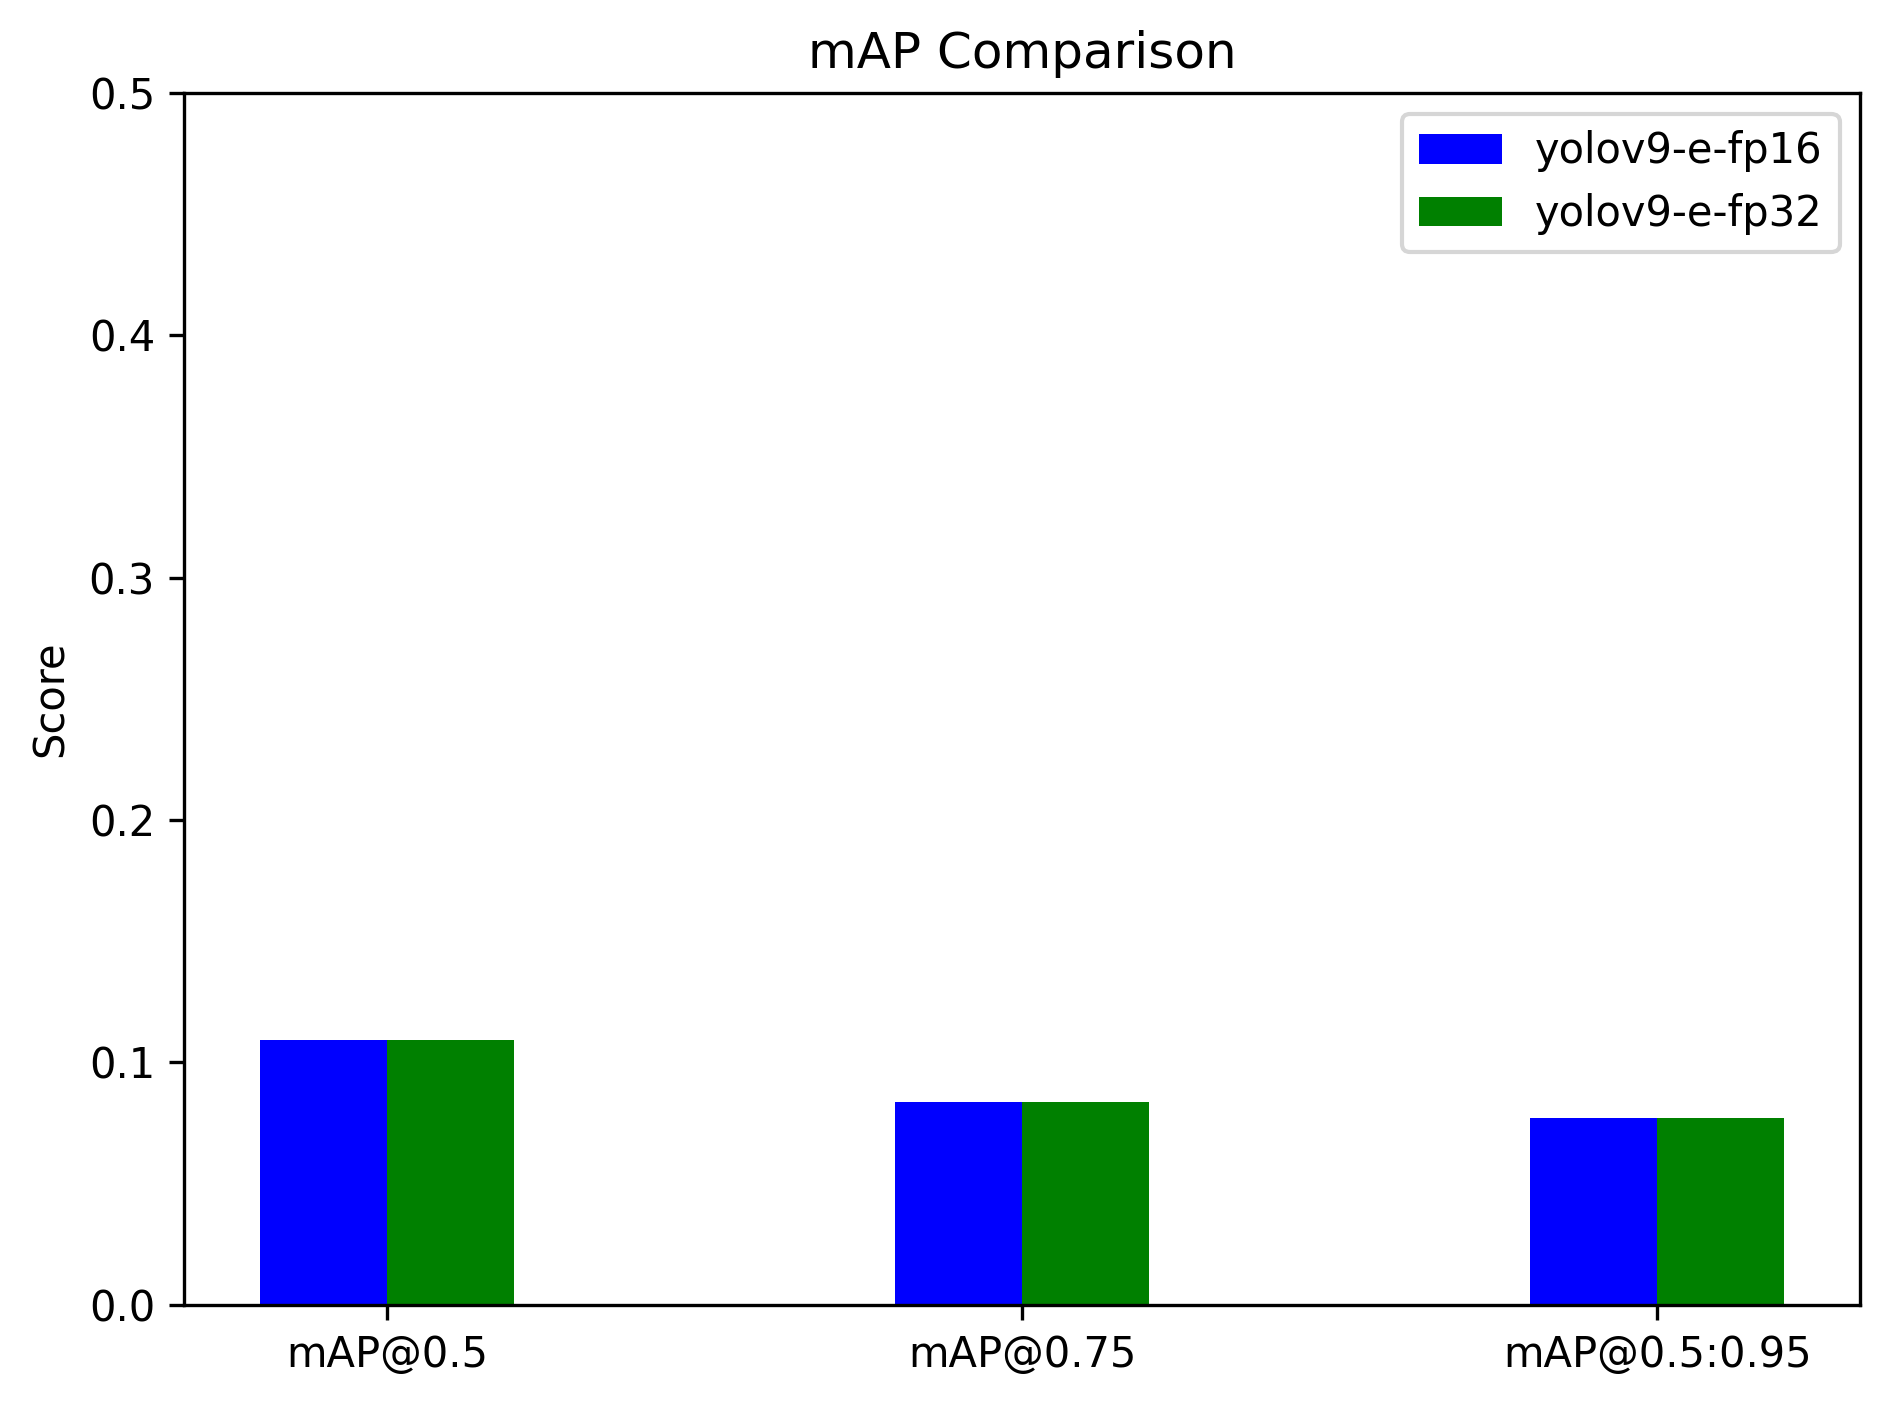
\includegraphics[width=3.75in,height=\textheight,keepaspectratio]{../images/map_comparison.png}

}

\caption{mAP (under different IOUs)}

\end{figure}%

\begin{figure}[H]

{\centering 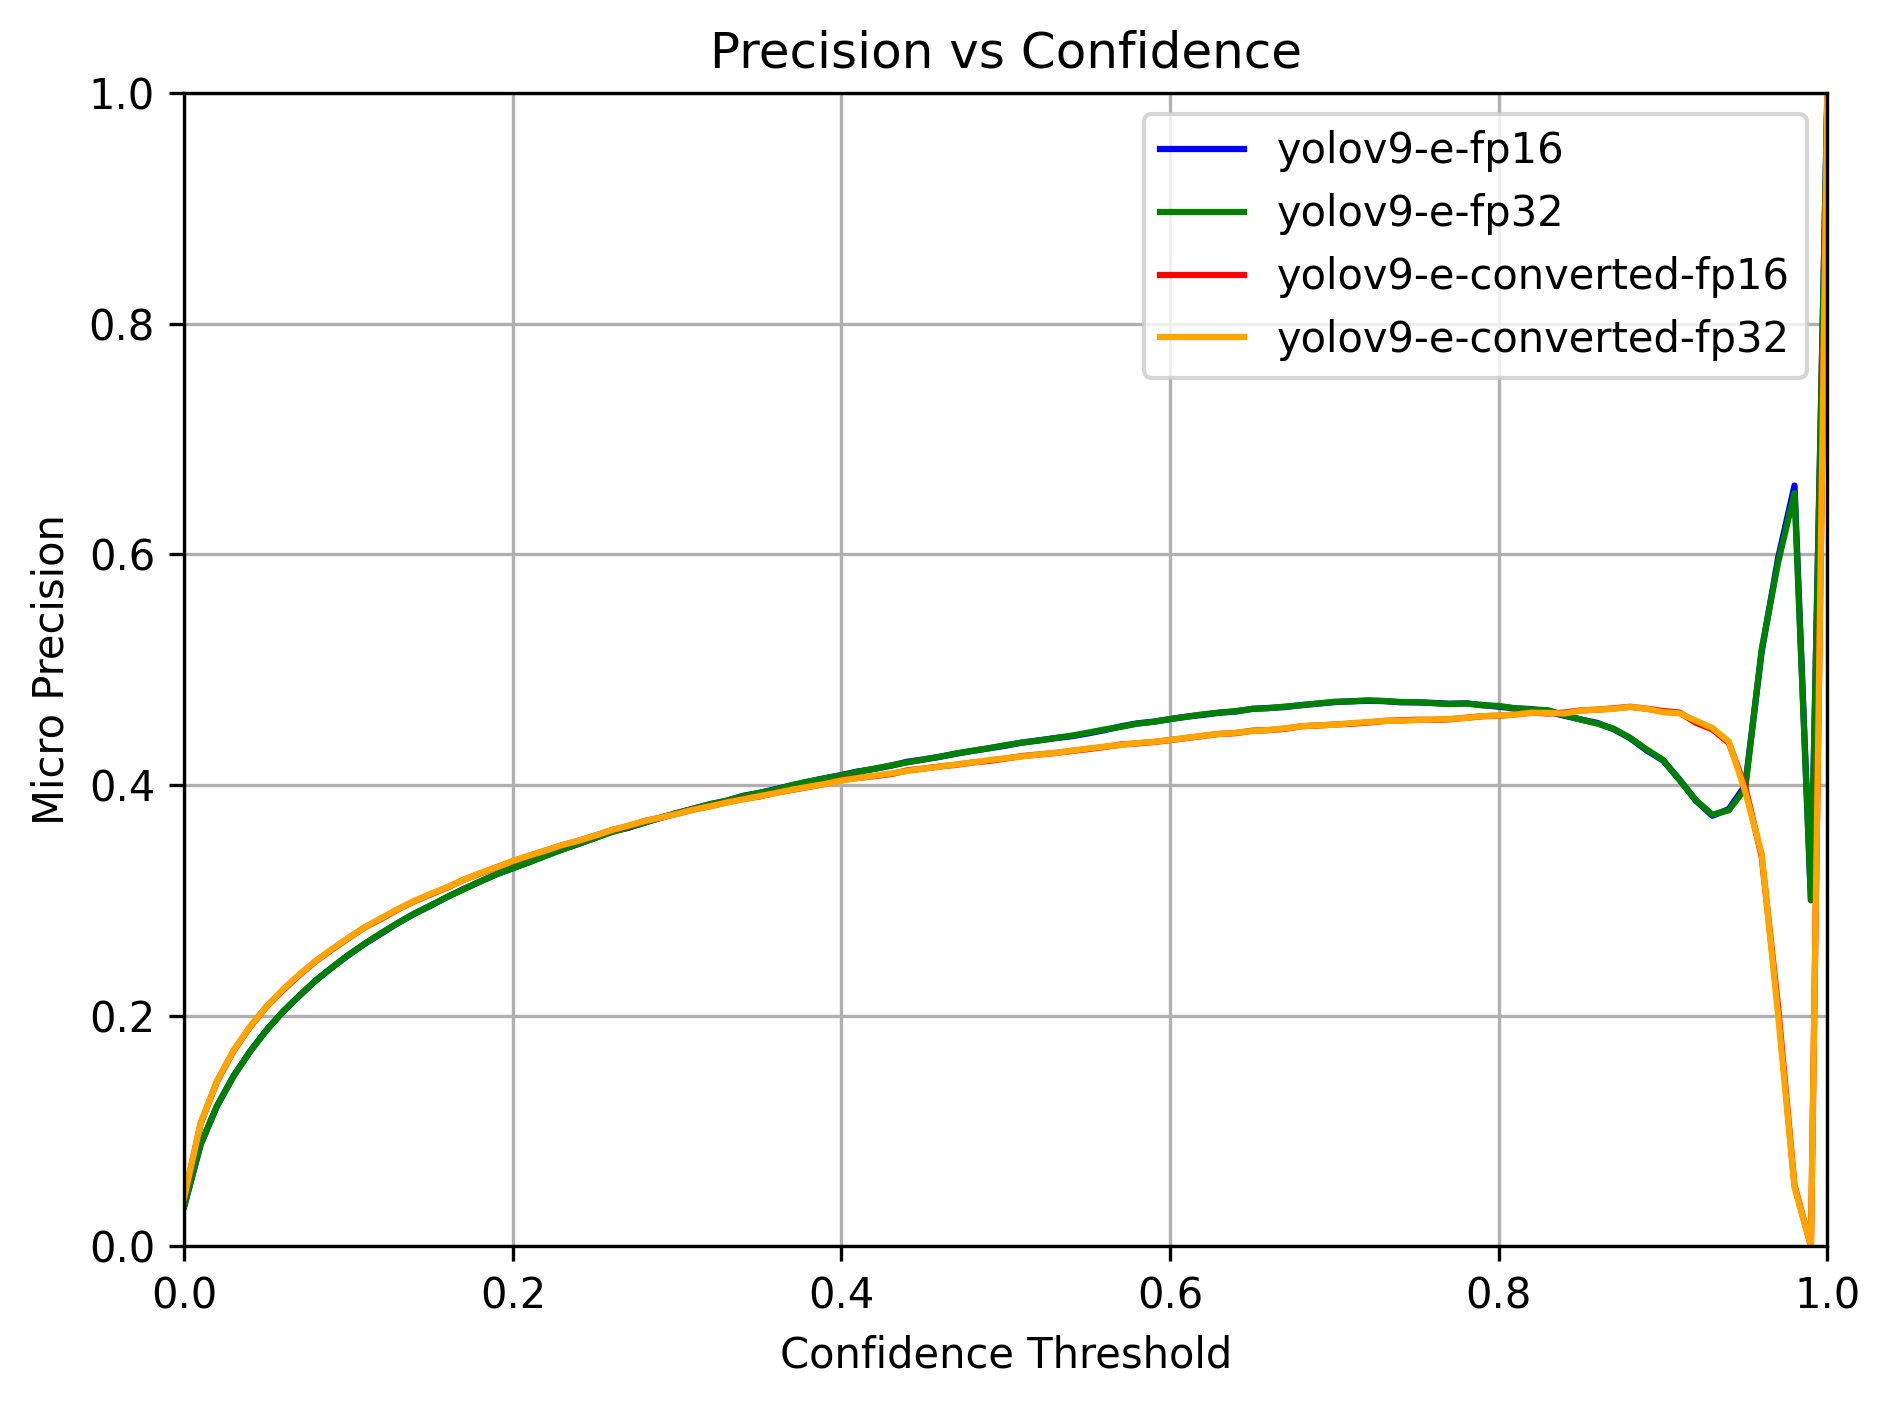
\includegraphics[width=3.75in,height=\textheight,keepaspectratio]{../images/precision_confidence_curve.png}

}

\caption{Precision - Confidence Curve}

\end{figure}%

\begin{figure}[H]

{\centering 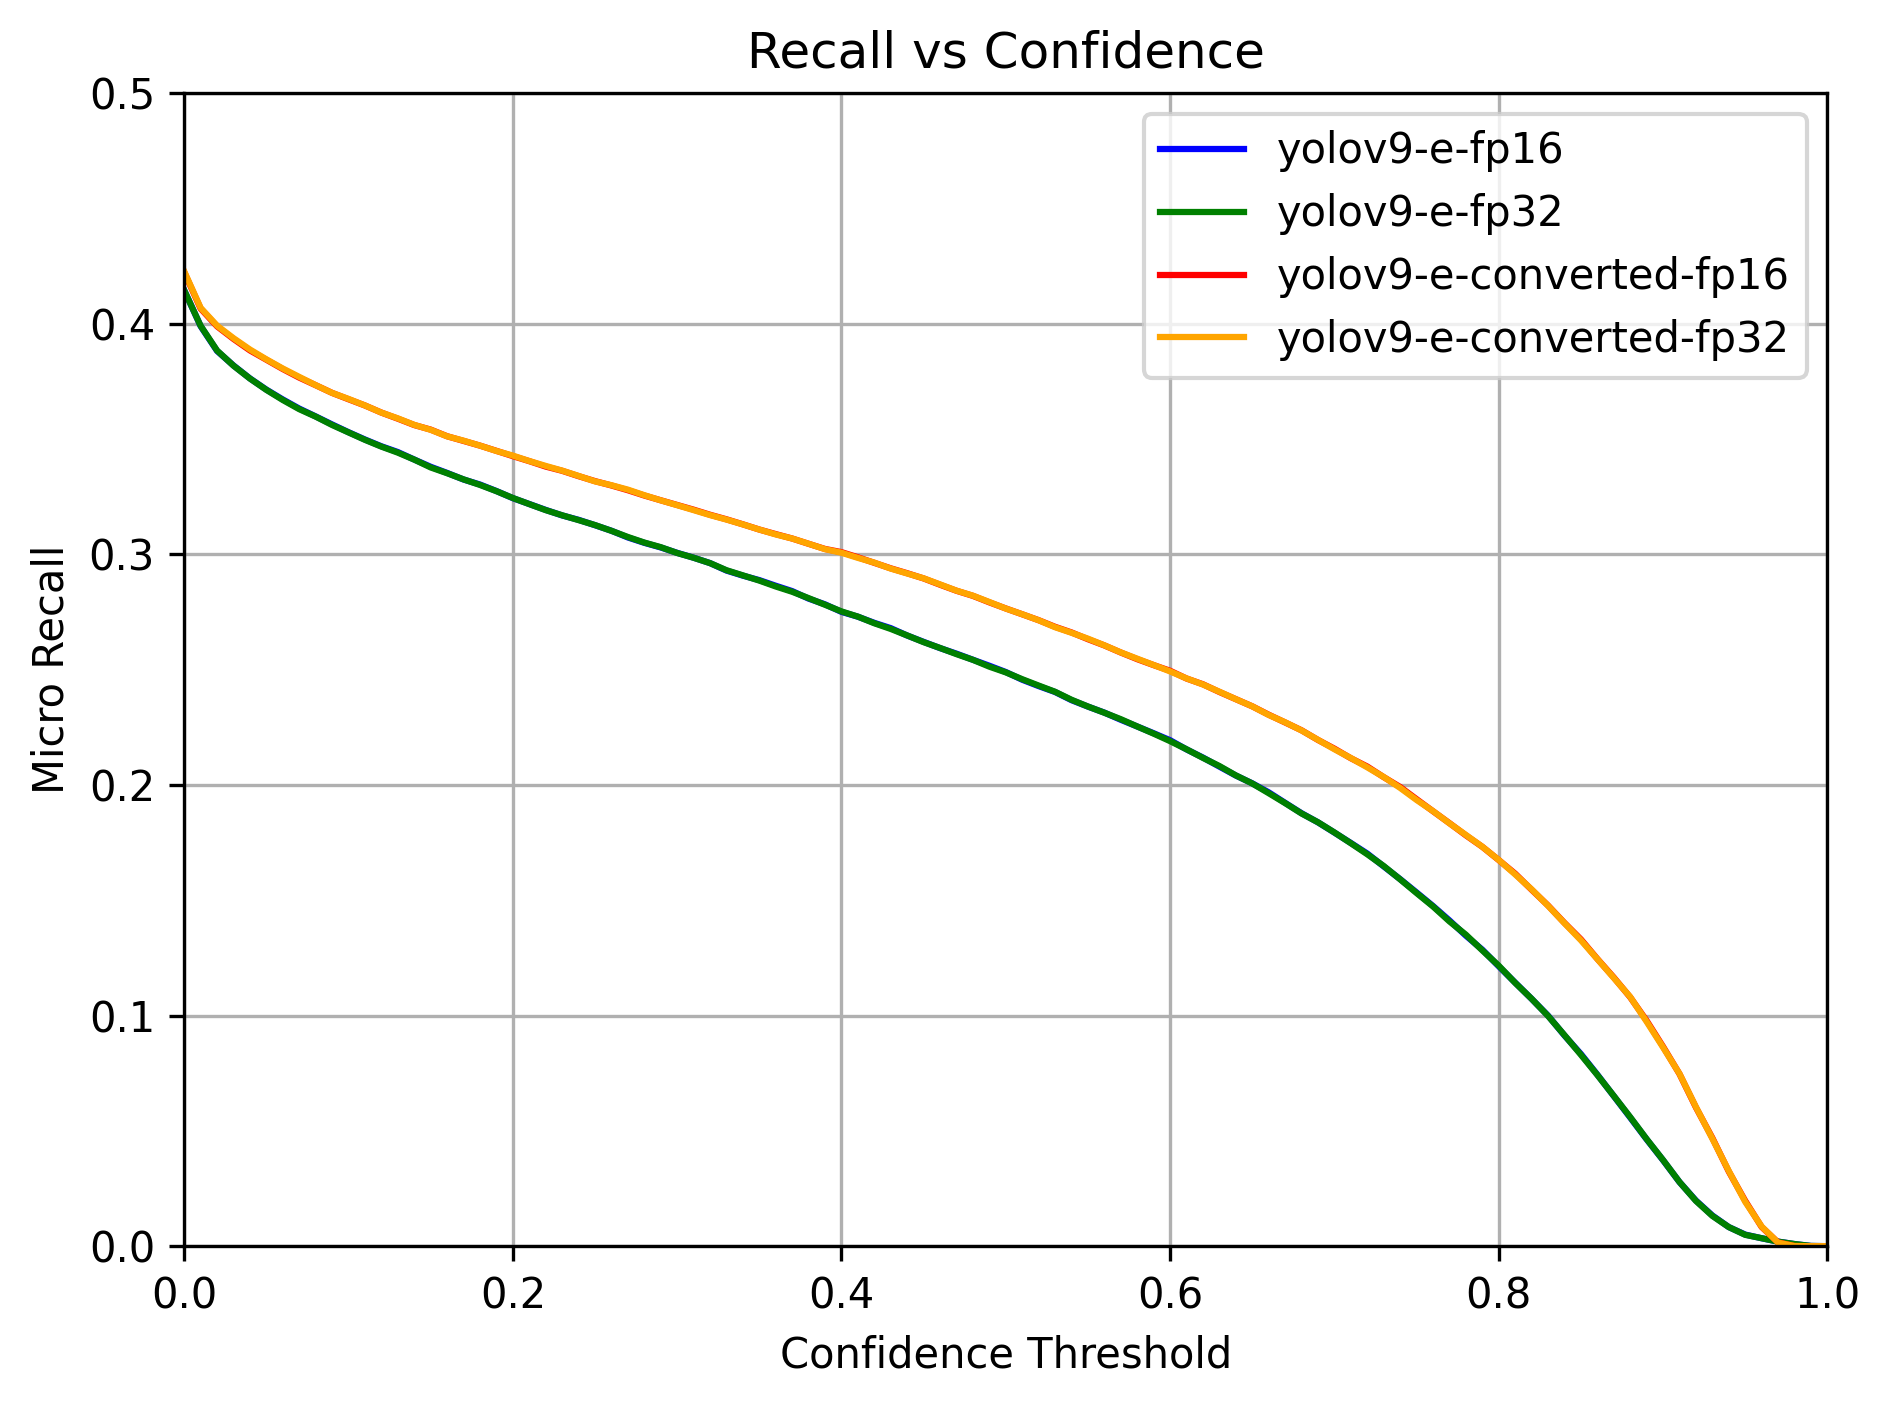
\includegraphics[width=3.75in,height=\textheight,keepaspectratio]{../images/recall_confidence_curve.png}

}

\caption{Recall - Confidence Curve}

\end{figure}%

\begin{figure}[H]

{\centering 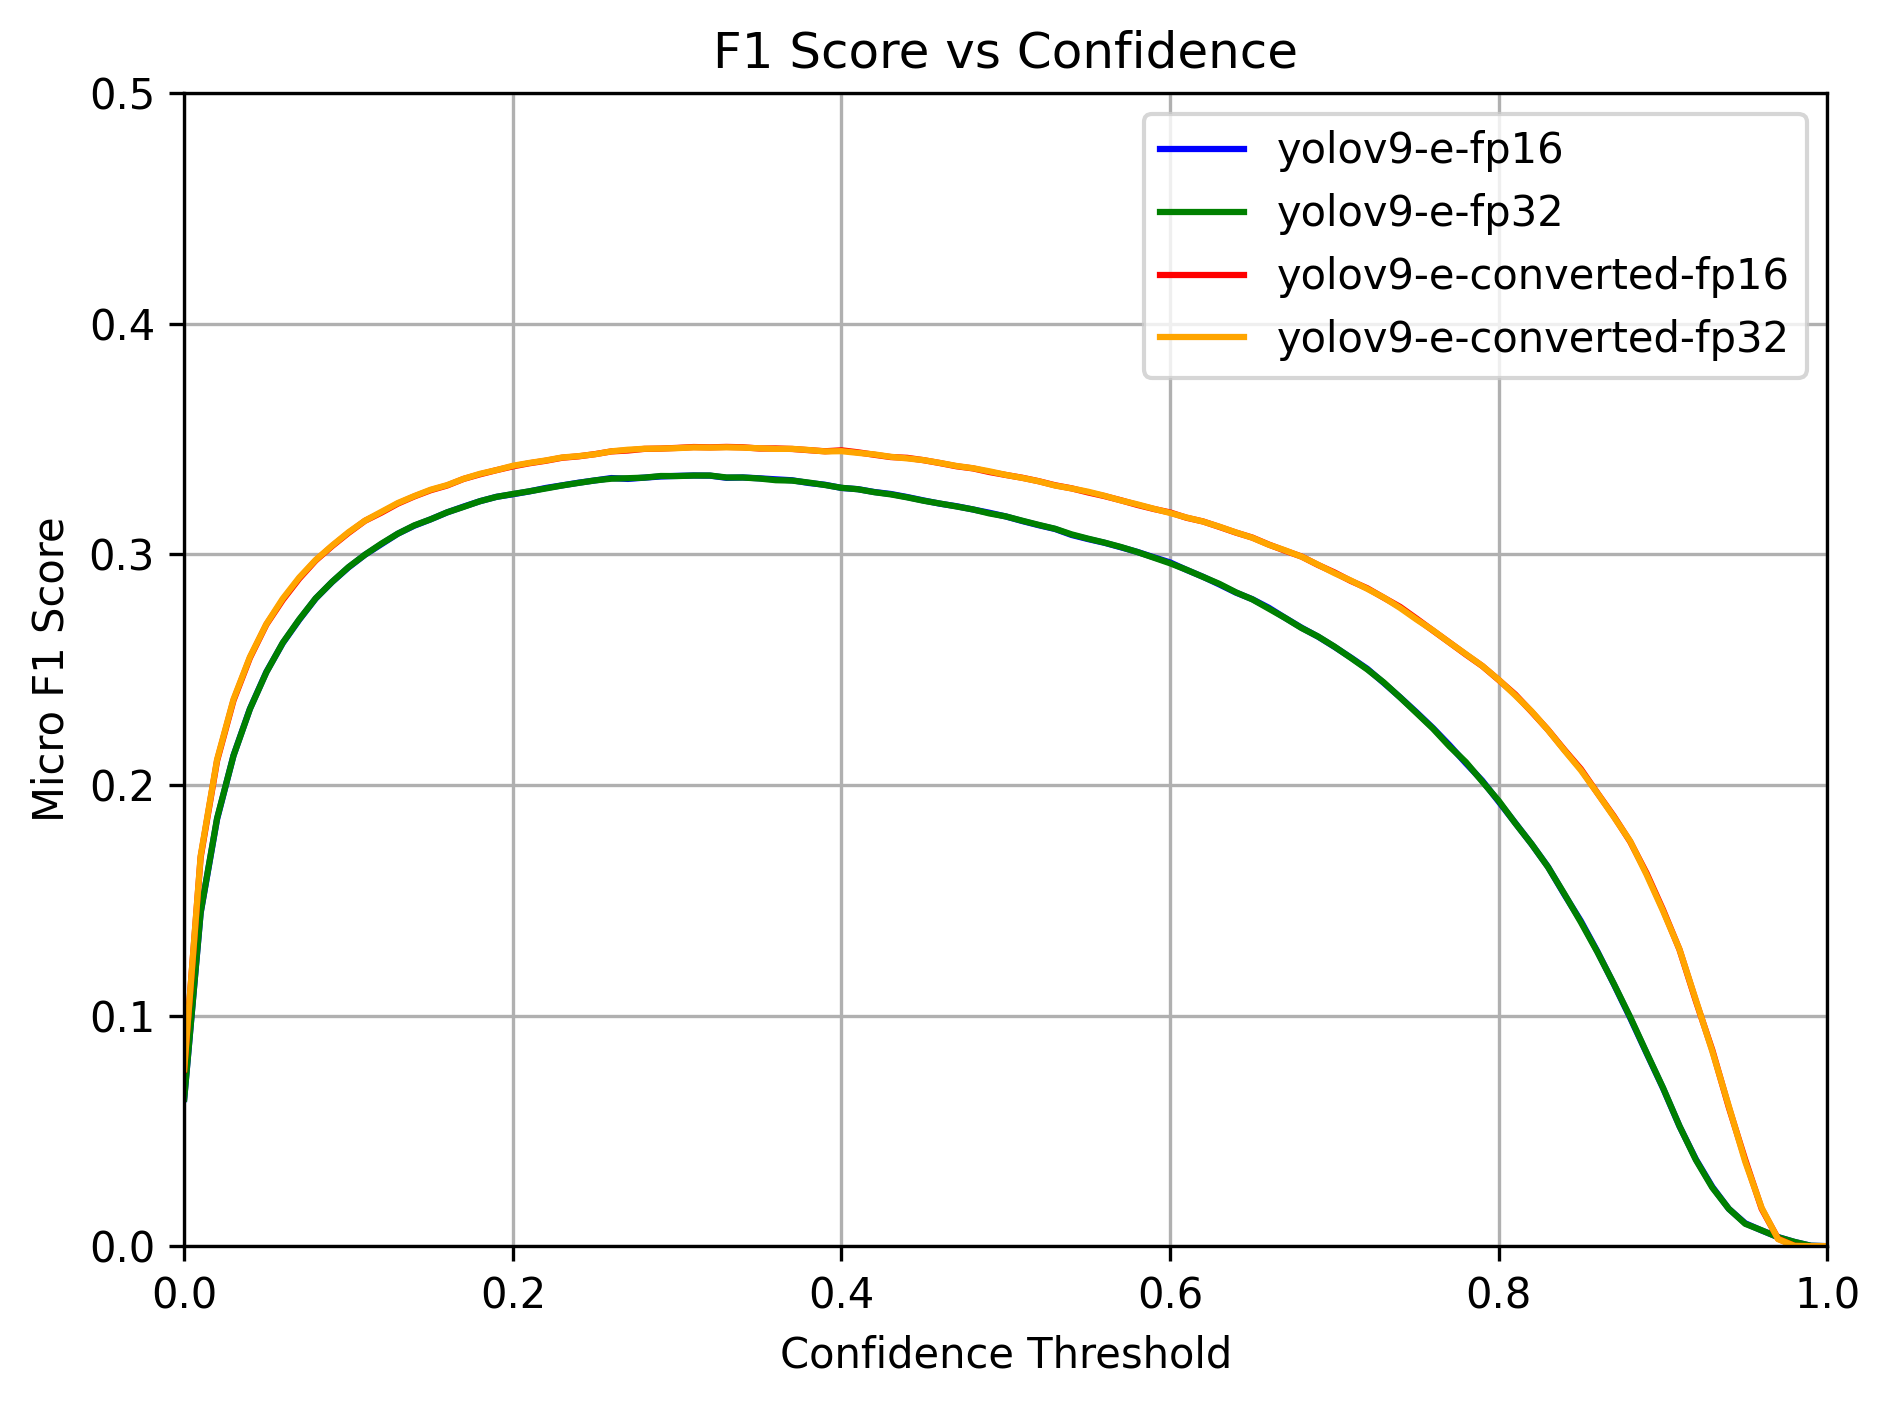
\includegraphics[width=3.75in,height=\textheight,keepaspectratio]{../images/f1_score_confidence_curve.png}

}

\caption{F1 Score - Confidence Curve}

\end{figure}%

\begin{figure}[H]

{\centering 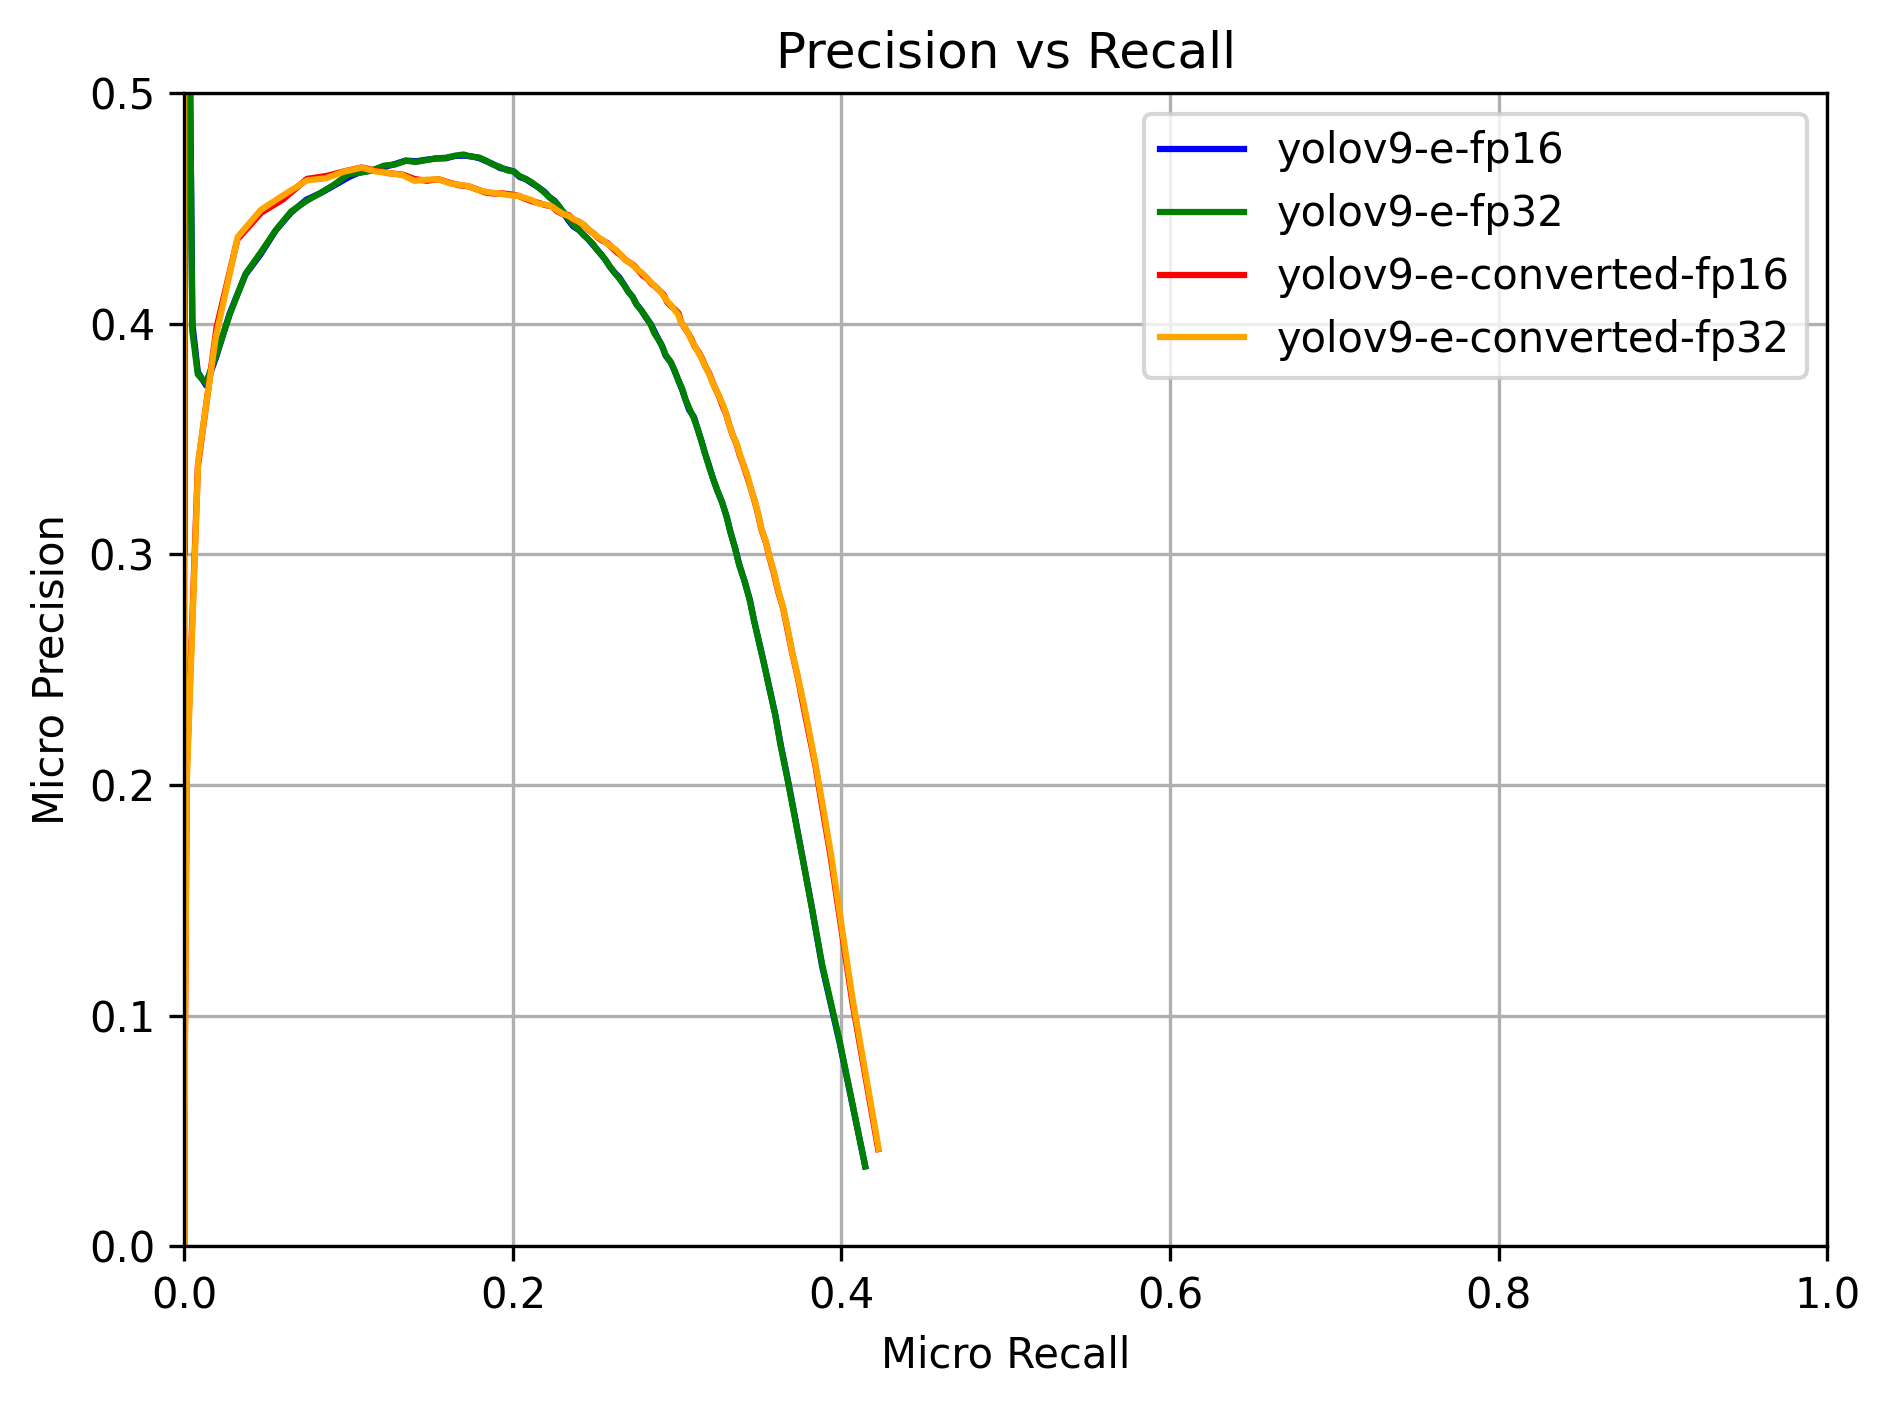
\includegraphics[width=3.75in,height=\textheight,keepaspectratio]{../images/precision_recall_curve.png}

}

\caption{Precision - Recall Curve}

\end{figure}%

While it may not be visible right away, we can see that FP16 and FP32
results for the same kind of model are overlapping in all curves. This
means that they both reach identical results(with minor changes after
the 4th floating digit). \newline With that said, \textbf{FP16 models
will be our choice of deployment} as they allow us to have the same
inference accuracy while significantly lowering inference time(higher
throughput).

\newpage{}

\subsection{3.2 Model Performance}\label{model-performance}

With the fact that FP16 models allow us to have same precision, while
being much faster at inference time, we will be having all further tests
made on FP16 models only. \newline Along with optimizing model
internals(the actual neural network)(using efficient code, fp16 models),
we need to have some tools to be able to boost the models to a higher
level of performance, and \textbf{NVIDIA TensorRT} solves just that.
NVIDIA TensorRT allows us to compile a model specific to our GPU
hardware, therefore very efficient with memory management inside the
GPU, giving us peak performance at almost no hard work. One of
TensorRT's main functions is allowing batch-processing of inputs,
therefore allowing us to get multiple results and process much more data
in less time. \newline Coupled with NVIDIA TensorRT, we also have
\textbf{NVIDIA Triton Server}, which is a platform used to serve those
models and run efficient inference on. All models are served through
HTTP/gRPC requests, and allow us to perform inference through those
protocols. Triton Server comes hand to hand with TensorRT, leveraging
all TensorRT advantages(batch-processing, multiple model instances
running at the same time), therefore boosting our performance even more.
\newline For the following experiment we have compiled our models with
TensorRT, specifically with dynamic inputs(Unlocking the
batch-processing features) and FP16(for lighter and faster models). We
have tested the model throughput for different amounts of concurrent
requests, to test how much we can squeeze out of our GPU. \newline
Experiment ran with the following environment specifications:

\begin{itemize}
\tightlist
\item
  CUDA 12.9
\item
  TensorRT 10.11.0
\item
  Triton Server 25.06
\item
  RTX 4070 GPU
\end{itemize}

\emph{Note} - The model we deployed on Triton Server uses a specific
config tailored to squeeze the best out of our model. It involves
dynamic batching, special GPU settings and more. Will be provided
alongside this document.

\begin{figure}[H]

{\centering 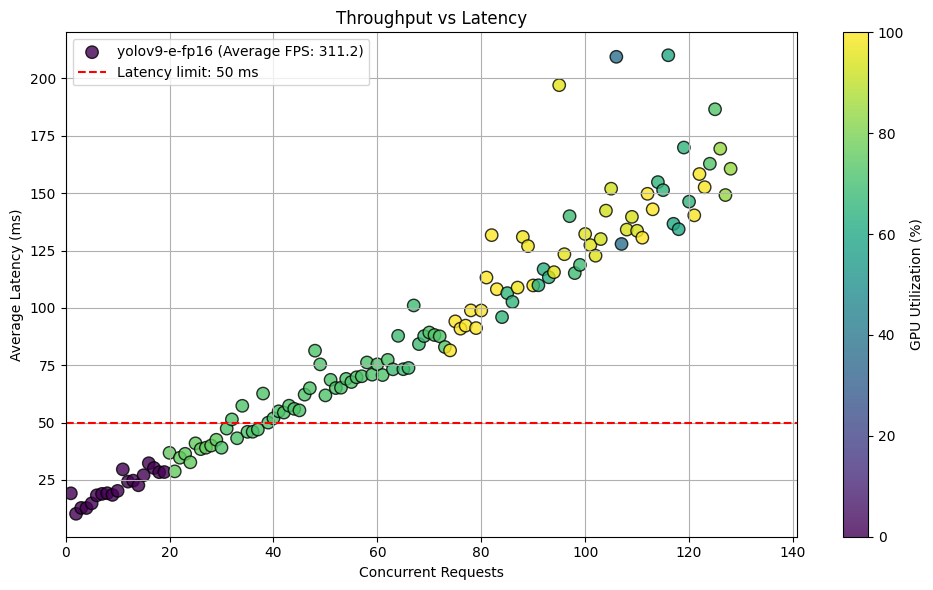
\includegraphics[width=4.30556in,height=\textheight,keepaspectratio]{../images/throughput_yolov9_e_fp16.png}

}

\caption{YOLOV9-e FP16 Throughput}

\end{figure}%

\begin{figure}[H]

{\centering 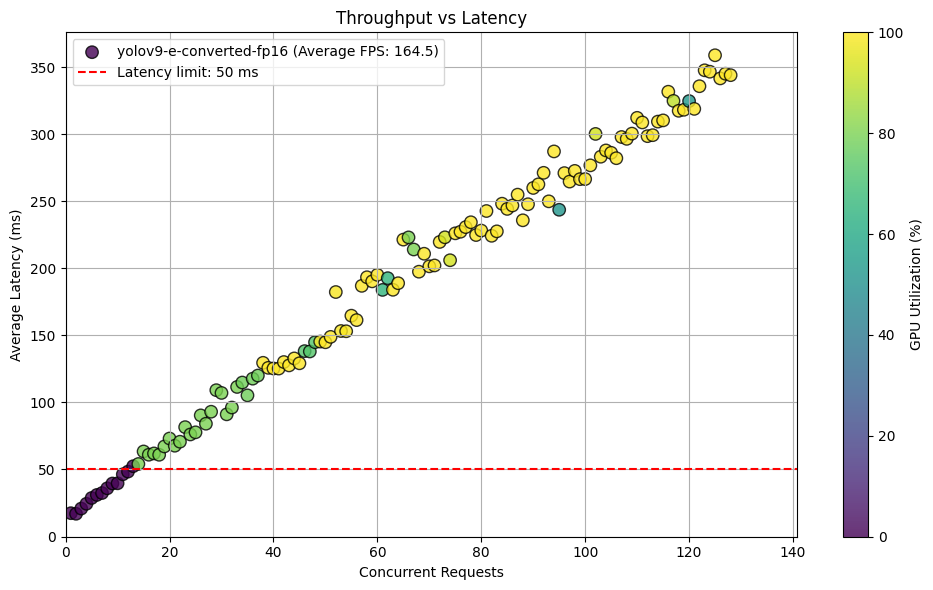
\includegraphics[width=4.30556in,height=\textheight,keepaspectratio]{../images/throughput_yolov9_e_converted_fp16.png}

}

\caption{YOLOV9-e-converted FP16 Throughput}

\end{figure}%

Each graph shows a model performance(``stress test'') under different
amounts of concurrent requests, essentially simulating our ``real-time
video'' scenario. Each dot represents a test conducted for X amount of
concurrent requests at once(X-axis), with the average latency we got per
request(Y-axis). The color indicates the GPU utilization at the
different points, with a scale allowing us to measure how well our GPU
is doing at every point. There is also an indication at the top left
corner, showing us how much FPS our model was able to serve per second.
With our real time video context, it will allow us to calculate how many
video streams our model will be able to serve at once: \[
\text{Total Streams} = \frac{\text{Model FPS}}{\text{Video Stream FPS}}
\]

Looking at our results, we can see that YOLOV9-e outperforms
YOLOV9-e-converted by almost double, while maintaining much lower GPU
utilization throughout the tests. This leads us to our final conclusion
- \textbf{YOLOV9-e-fp16 will be our model of choice} for building the
real-time video inference application.

\subsection{3.1 Architecture overview}\label{architecture-overview}

\begin{figure}[H]

{\centering 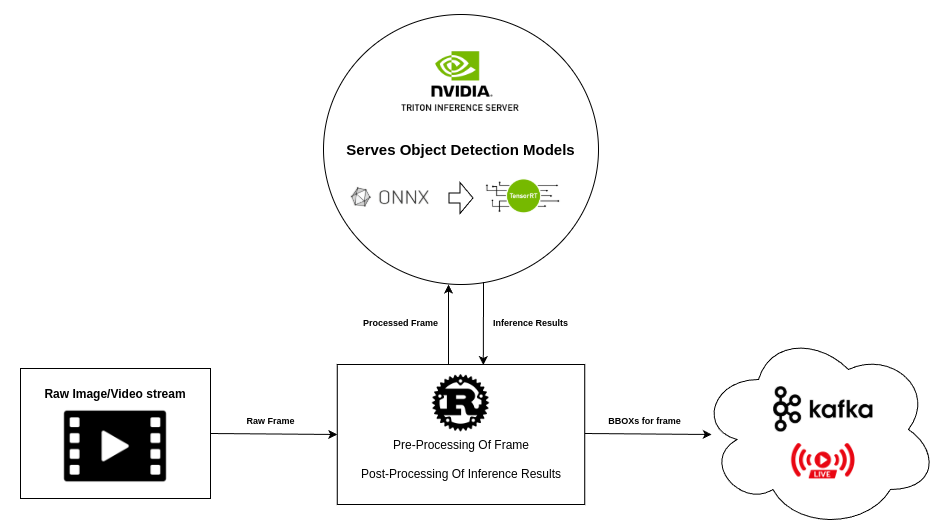
\includegraphics[width=4.44444in,height=\textheight,keepaspectratio]{../images/architecture.png}

}

\caption{Architecture for a real time video inference system}

\end{figure}%

Having our model pushed to it's limit is really great, but we also need
a steady system to back it up. We must build a strong, low latency
inference system, that doesn't create an overhead for pre-processing
video input or post-processing model output, and allows us to serve
inference results at near model time. for that we have two main options:

\begin{itemize}
\tightlist
\item
  \textbf{Python} - Has a very rich ML/processing tools such as pytorch,
  numpy, openCV, numba and much more, allowing us to run code in times
  close to C language. Having said that, it has many downsides, which we
  should take in mind:

  \begin{itemize}
  \tightlist
  \item
    Poor optimization - Python is not a low level programming language,
    therefore has many overhead components that hurt runtime(garbage
    collector, datatypes) and prevent us from getting instant response.
  \item
    Poor Multi-Threading - Running multiple threads(for multiple video
    streams for example) is very limited, as Python's GIL(Global
    Interpreter Lock) prevents us to run more than one python bytecode
    at a given time. Even with multithread packages(i.g. threading),
    will have to wait in queue for GIL to finish - not ideal for real
    time scenarios.
  \end{itemize}
\item
  \textbf{Rust} - Has a growing set of ML tools, such as openCV,
  ndarray(Numpy-like) and more, providing sufficient tools in our case.
  Rust has multiple upsides in case of real time inference:

  \begin{itemize}
  \tightlist
  \item
    C-like performance - Rust is very efficient, having no overhead
    components(No garbage collector) and other datatypes that can hurt
    runtime, rust allows us to write code in high level syntax with low
    level performance. Great for achieving real-time computations.
  \item
    Real multi-threading - Rust allows us run our program in real
    parallel, on multiple cores at a time natively. This allows us to
    serve multiple streams seperately without them depending on each
    other to finish running.
  \end{itemize}

  With that said, rust has a rather steep learning curve, and it takes
  time for an average programmer to be able to write production grade
  code.
\end{itemize}

With that said, \textbf{Rust will be our language of choice}, having its
capabilities overcome Python's, and with the idea of having our system
be stable, fast and reliable over time.




\end{document}
